Тестирование  на парах модельных изображений и на изображениях поверхностях реальных образцов.
\subsection{Образцы изображений}
\subsubsection{Модельные изображения}

В качестве образцов брались наборы изображений из интернет ресурса ``Society for Experimental Mechanics (sem.org)'' описание текстур находится в таблице \ref{tab:set_image}, текстуры изображены на рисунке \ref{pic:gray_mix}.

\begin{longtable}[h!]{|m{0.45\textwidth}|m{0.12\textwidth}|m{0.11\textwidth}|m{0.08\textwidth}|m{0.1\textwidth}|}
\caption{Описание модельных изображений}
\label{tab:set_image}
\\ \hline
Серия & Диапазон яркостей 	& Уровень шума & Сдвиг (px) &  Размеры \\ \hline
Модель многослойного изображения & 0-188 & Нет & 1-20 &  510x510 \\ \hline
Модель спекла & 0-188 & Нет & 1-70 &  512x512 \\ \hline
Модель высокий контраст & 10-240 & Низкий  & 0.1-1 & 487x325 \\ \hline
Prosilica Bin  & 10-156 & Низкий  & 0.1-1 & 487x325 \\ \hline
Strain Gradient & 20-185 	& Средний  & 0.01-1 & 512x512 \\ \hline
Strain Gradient & 30-225 	& Средний  & 0.01-1 & 512x512 \\ \hline
\end{longtable}

\subsubsection{Реальные отснятые изображения}

Реально отснятые изображения предоставлены сотрудником ИФПМ СО РАН. 

На первой серии (рисунок \ref{pic:al_deform}) изображён металлический образец из авиационного алюминиевого сплава Д16АТ нагружавшиеся на механической испытательной машине ИМАШ-2078 в условиях одноосного статического растяжения. Размеры предоставленных изображений 1920х1280 пикселей.
\begin{figure}[ht]
\center{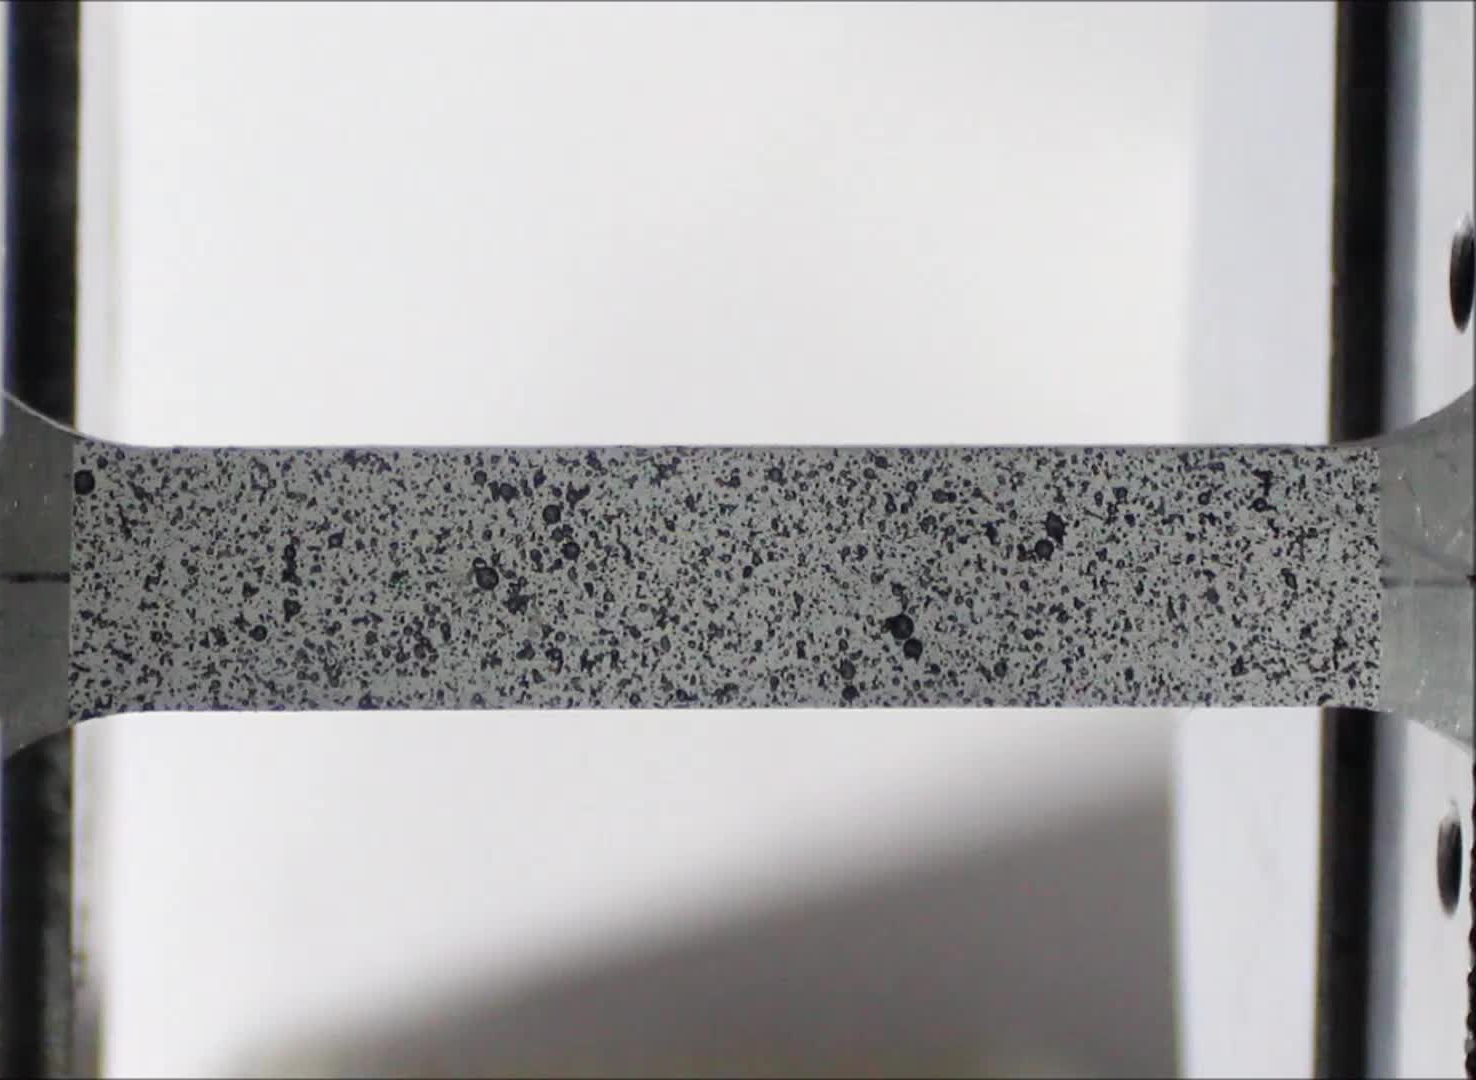
\includegraphics[width=0.6\linewidth]{al_deform}}
\caption{Растяжение пластины алюминия Д16АТ}
\label{pic:al_deform}
\end{figure}

На второй серии (рисунок \ref{pic:carbon_deform}) изображён углерод-углеродный композиционный материал. Образец испытывали на одноосное статическое растяжение на электро-механической машине Instron 5582 со скоростью перемещения подвижного захвата 0,3 мм/мин.
\begin{figure}[h!]
\center{\includegraphics[width=0.6\linewidth]{carbon_deform}}
\caption{Углерод-углеродный композиционный материал}
\label{pic:carbon_deform}
\end{figure}

Фотографирование поверхности осуществляли с помощью фотокамеры Canon EOS 550D, оснащённой длиннофокусным объективом Canon EF-S 100-400mm 1/4-5.6 IS.

\subsection {Оценка быстродействия}
Для проведения расчётов использовали ПЭВМ со следующими характеристиками:

Аппаратная составляющая:
\begin{itemize}
\item процессор Intel(R) Core(TM) i3 370M @ 2,4 ГГц, 64-бит;
\item оперативная память 4 Гб, 1067 МГц;
\item материнская плата Aspire 573
\item жёсткий диск SSD Smartbuy 120 Гб;
\item файловая система ext4, 107 Гб.
\end{itemize}
Программная составляющая:
\begin{itemize}
\item операционная система Linux Mint 3.19-18;
\item версия cmake 3.2.1;
\item версия QMake 3.0 \& Qt version 5.2.1;
\item версия компилятора gcc (Ubuntu 4.8.2-19ubuntu1) 4.8.2;
\item оболочка для среды рабочего стола Cinnamon 2.4.8.
\end{itemize}

Для исследования быстродействия и помехоустойчивости алгоритмов были использованы описанные ранее серии изображений.

\subsection{Тестирование программного обеспечения}
\subsubsection{Тестирование на модельных изображениях}

Для первого раза используем изображения из серии Grey texture, представленные на рисунке \ref{pic:gray_mix} а). Они имеют сдвиг по оси $x$ на один пиксель влево, по $y$ сдвиг отсутствует.

\begin{figure}[h!]
\center{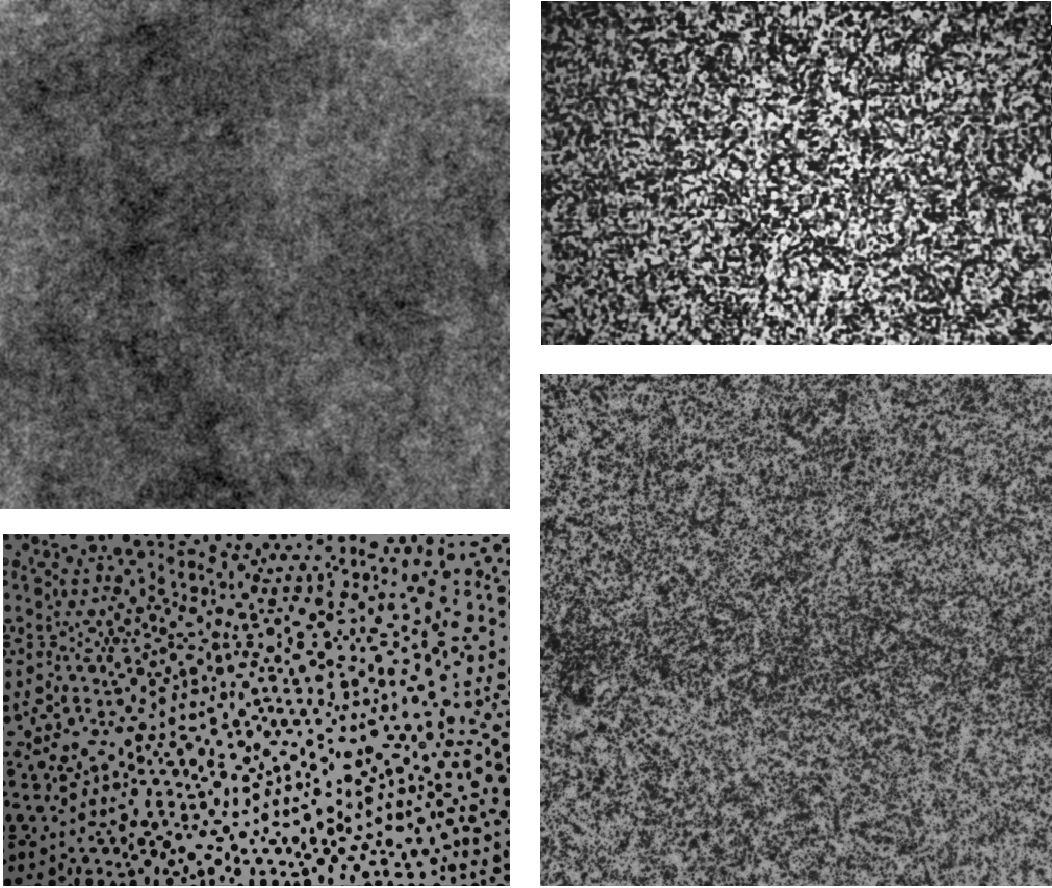
\includegraphics[width=0.9\linewidth]{gray_mix}}
\caption{Тестовая серия изображений: Grey set, High contrast, Sample6, Sample10, Sample11b, Grey set V2 }
\label{pic:gray_mix}
\end{figure}

Результатом работы ПО, как описано в первом разделе, является векторное поле и поля деформации твёрдого тела представленное на рисунке \ref{pic:gray_set_out}.

\begin{figure}[h!]
\center{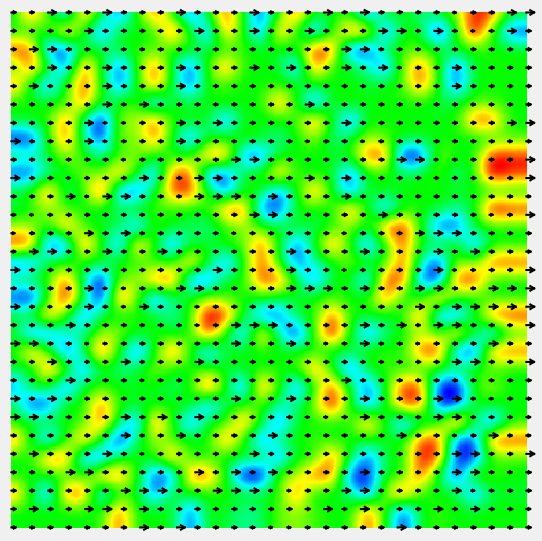
\includegraphics[width=0.6\linewidth]{gray_set_out}}
\caption{Поле смещений и деформации твёрдого тела}
\label{pic:gray_set_out}
\end{figure}

\begin{figure}[h!]
\center{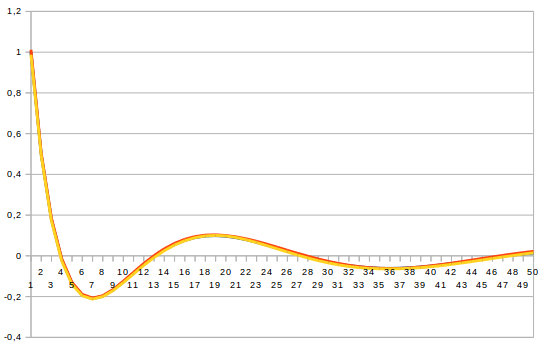
\includegraphics[width=0.6\linewidth]{gray_set_func_iteration}}
\caption{Зависимость уровня ошибки, от числа итераций}
\label{pic:gray_set_func_iteration}
\end{figure}

\subsubsection{Тестирование на экспериментально полученных изображения}
В данном разделе приведены результаты тестирования разрабатываемого программного обеспечения на изображениях поверхностей реальных образцов.

\subsection{Исследование метода интерполяции}

\subsection{Исследование размера окна поиска}
\begin{figure}[h!]
\center{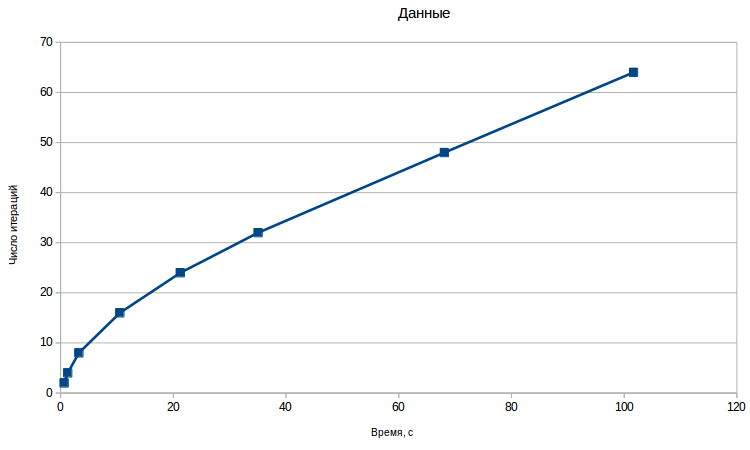
\includegraphics[width=0.6\linewidth]{images/window_time.png}}
\caption{Время работы программы, в зависимости от размера окна}
\label{pic:window_time}
\end{figure}

\begin{figure}[h!]
\center{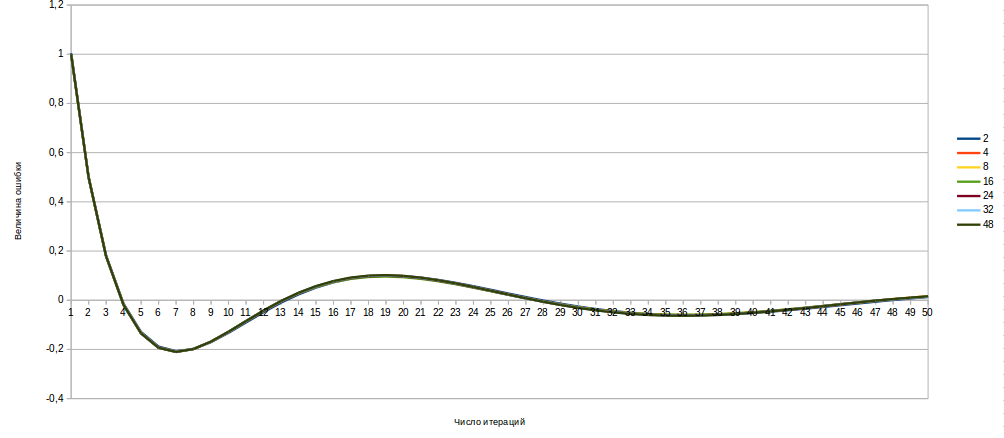
\includegraphics[width=0.6\linewidth]{images/window_size.png}}
\caption{Уровень ошибки, в зависимости от размера окна}
\label{pic:window_size}
\end{figure}
